% To rebuild the .pdf from this source, use something like the following
%	latex quickref.tex
%	dvips -t letter -f -Pcmz < quickref.dvi >| quickref.ps
%	ps2pdf -sPAPERSIZE=letter quickref.ps
\documentclass[12pt]{article}
\usepackage[utf8]{inputenc}
\usepackage{lscape}
\usepackage{setspace}
\usepackage{graphicx}
\usepackage{multicol}
\usepackage[normalem]{ulem}
\usepackage[catalan]{babel}
\usepackage{color}
\usepackage{hyperref}

\textheight=9in
\textwidth=7.5in
\headheight=0pt
\headsep=0pt
\topmargin=0in
\oddsidemargin=-0.4in
\evensidemargin=-0.6in
\parindent=0pt
\parsep=1pt
\pagestyle{empty}

\date {}

\makeatother

\begin{document}
	\begin{landscape}

%	\textit{Dan Kuester's all-leather}

	\begin{center}
	\begin{minipage}[m]
		{1in}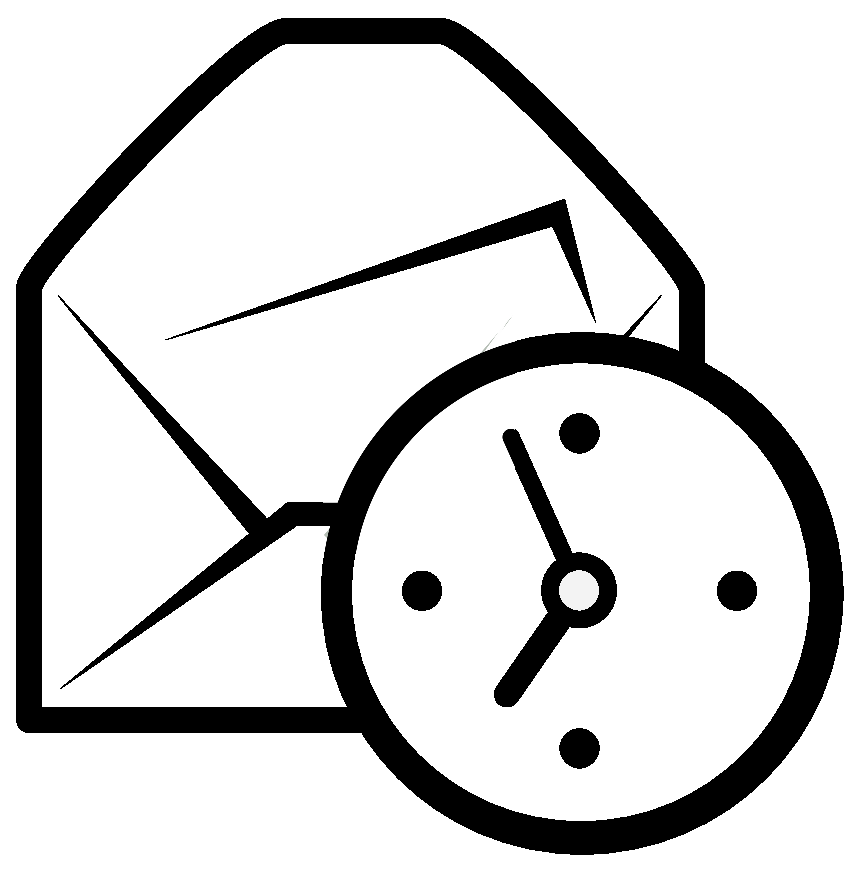
\includegraphics[height=0.9in]{../evolution-logo.eps}\hspace{5mm}
	\end{minipage}
	\hspace{5mm}
	\textbf{\Huge{Referència ràpida de l'Evolution}}
	\end{center}

	\begin{center}
	\begin{multicols}{2}
	\section*{Global}
	\begin{tabular*}{5in}{rp{1.5in}}
		\textit{\textbf{Components}}		&					\\
		Correu					& \textbf{Ctrl+1}			\\
		Contactes				& \textbf{Ctrl+2}			\\
		Calendaris				& \textbf{Ctrl+3}			\\
		Tasques					& \textbf{Ctrl+4}			\\
		\vspace{1.5mm}
		Anotacions					& \textbf{Ctrl+5}			\\
		\textit{\textbf{Controls}}		&					\\
		Element nou en el mode actual		& \textbf{Ctrl+N}			\\
		Commuta el focus entre subfinestres		& \textbf{F6}				\\
		Neteja la barra de cerca			& \textbf{Majús+Ctrl+Q}			\\
		Tanca la finestra				& \textbf{Ctrl+W}			\\
		Obre una finestra nova				& \textbf{Majús+Ctrl+W}			\\
		\vspace{1.5mm}
		Surt de l'Evolution				& \textbf{Ctrl+Q}			\\
		\textit{\textbf{Selecció}}		&					\\
		Imprimeix la selecció				& \textbf{Ctrl+P}			\\
		Desa la selecció				& \textbf{Ctrl+S}			\\
		Suprimeix la selecció			& \textbf{Supr} o \textbf{Retrocés}	\\
		Mou els correus/contactes a la carpeta		& \textbf{Majús+Ctrl+V}			\\
		Copia els correus/contactes a la carpeta		& \textbf{Majús+Ctrl+Y}			\\
	\end{tabular*}
	\section*{Components de contactes/anotacions}
	\begin{tabular*}{4in}{rp{1.5in}}
		\textit{\textbf{Ordres generals}}	&					\\
		Contacte nou				& \textbf{Majús+Ctrl+C}			\\
		Llista de contactes nova			& \textbf{Majús+Ctrl+L}			\\
		Anotació nova				& \textbf{Majús+Ctrl+O}			\\
	\end{tabular*}
%	{\\ \vspace{5mm} \footnotesize \textit{* denotes the feature may not be implemented yet}}
	\section*{Component de correu}
	\begin{tabular*}{4in}{rp{1.5in}}
		\textit{\textbf{Ordres generals}}	&					\\
		Missatge nou				& \textbf{Majús+Ctrl+M}			\\
		\vspace{1.5mm}
		Envia/rep missatges			& \textbf{F9}				\\
		\textit{\textbf{Selecció}}		&					\\
		Aplica els filtres				& \textbf{Ctrl+Y}			\\
		Obre en una finestra nova 			& \textbf{Retorn} o \textbf{Ctrl+O}	\\
		\vspace{1.5mm}
		Reenvia la selecció			& \textbf{Ctrl+F}			\\
		\textit{\textbf{Subfinestra de la llista de missatges}}	&					\\
		Missatge no llegit següent			& \textbf{.} o \textbf{]}		\\
		\vspace{1.5mm}
		Missatge no llegit anterior			& \textbf{,} o \textbf{[}		\\
		\textit{\textbf{Subfinestra de previsualització}}		&					\\
		Respon al remitent				& \textbf{Ctrl+R}			\\
		Respon a la llista				& \textbf{Ctrl+L}			\\
		Respon a tots els destinataris 		& \textbf{Majús+Ctrl+R}			\\
		Desplaça't cap amunt				& \textbf{Retrocés}			\\
		Desplaça't cap avall				& \textbf{Espai}			\\
	\end{tabular*}
	\section*{Components de calendaris/tasques}
	\begin{tabular*}{4in}{rp{1.5in}}
		\textit{\textbf{Ordres generals}}	&					\\
		Cita nova				& \textbf{Majús+Ctrl+A}			\\
		Reunió nova				& \textbf{Majús+Ctrl+E}			\\
		\vspace{1.5mm}
		Tasca nova				& \textbf{Majús+Ctrl+T}			\\
%		\vspace{1.5mm}
%		Expunge/Purge old schedules		& \textbf{Ctrl+E}			\\
		\textit{\textbf{Navegació}}		&					\\
		Vés a la data d'avui				& \textbf{Ctrl+T}			\\
		Vés a una data				& \textbf{Ctrl+G}			\\
	\end{tabular*}
	\end{multicols}
	\end{center}
	\end{landscape}
 \end{document}
